\documentclass[11pt,a4paper,twocolumn]{article}
\usepackage[utf8]{inputenc}
\usepackage[T1]{fontenc}
\usepackage{amsmath}
\usepackage{amssymb}
\usepackage{amsfonts}
\usepackage{graphicx}
\usepackage[spanish]{babel}
\usepackage{tcolorbox,booktabs,fourier,tabularx,wrapfig,multicol,caption, subcaption,tikz,fancyhdr}

\usepackage[left=1.5cm,right=2cm,top=2cm,bottom=2cm]{geometry}

\graphicspath{{./imageneselectro/}}


\author{Franco Guardiani, Valentin Franzoi, Daiana Polo}
\title{
\includegraphics[width=.3\textwidth]{utn} \\ \textsc{Electrotecnia} \\ \textsl{Resumen teórico} \\ }
\date{2022}

%Comando título de cada unidad
\newcommand{\unidad}[2]{\begin{center}
		\fontsize{10}{10}\selectfont\color{gray!50!black}\scshape Unidad #1 \\
		\fontsize{14}{14}\selectfont \scshape #2
\end{center}}

\fancyfoot[C]{}
\fancyfoot[R]{\thepage}
\fancyhead[R]{\textsc{Electrotecnia}}
\renewcommand{\headrulewidth}{0pt}
\fancyfoot[L]{Franco Guardiani, Valentin Franzoi, Daiana Polo}

\begin{document}
	\pagestyle{fancy}
	\maketitle
	\section*{Nomenclatura}
	\begin{tabular}{r l}
		$R$ & Resistencia \\
		$C$ & Capacitancia \\
		$L$ & Inductancia \\
		$i$ & Corriente \\
		$v$ & Voltaje \\
		$w$ & Energía almacenada \\
		$j$ & Unidad imaginaria \\
		$t$ & Tiempo \\
		$LTK$ & Ley de Kirchhoff para la tensión \\
		$LCK$ & Ley de Kirchhoff para la corriente \\
		$Z$ & Impedancia \\
		$X_{C}$ & Reactancia capacitiva \\
		$X_{L}$ & Reactancia inductiva \\
		$Y$ & Admitancia\\
		$G$& Conductancia\\
		$B$ & Suceptancia\\
		$\tau$ & Constante de tiempo \\
		$\alpha$ & Factor de amortiguamiento \\
		$\omega_{0}$ & Frecuencia natural no amortiguada \\
		$\omega_{d}$ & Frecuencia natural amortiguada \\
		
		
		
	\end{tabular}
	
	\newpage
	
	\section*{Conceptos}
	
	Example: 
	
	\textbf{Corriente eléctrica:} es el movimiento ordenado de cargas libres, normalmente de electrones, a través de un material conductor en un circuito eléctrico.
	
	\textbf{Circuito monofásico:} aquel en el que se toma una linea (R,S,T) y un neutro.
	
	\textbf{Fasor:} Un número complejo que representa la amplitud y la fase de una senoide.
	
	\textbf{Impedancia:} de un circuito es la razón entre la tensión fasorial \textbf{\textit{V}} y la corriente fasorial \textbf{\textit{I}}, [$\Omega$]
	\newpage
	
	\unidad{1}{Teoría Elemental de los Circuitos}
	
	\begin{tabular}{r | l}     \vspace{.2cm}
		Ley de Omh & $I=\dfrac{V}{R}$\\  \vspace{.2cm}
		Fasores & $Z=R+j(X_{L}-X_{C})$ \\  \vspace{.2cm}
		Elementos pasivos & Resistor, inductor, capacitor \\  \vspace{.2cm}
		Elementos activos & Fuente, generador\\
		
	\end{tabular}
	
	\unidad{2}{Respuesta Natural}

	La respuesta natural o transitoria de un circuito se refiere al comportamiento (en términos de tensiones y corrientes) del circuito, sin fuentes externas de excitación. Se extingue con el tiempo
	
	\begin{center}
		\large\textsc{\textbf{Circuitos de primer orden}}
	\end{center}
	
	\textsl{Concepto}
	
	\textbf{Circuito RL sin fuente} 
	\begin{center}
		\begin{tabular}{r | l} \vspace{.2cm} 
		LTK & $0=iR+L \dfrac{di}{dt}$ \\ \vspace{.2cm}
		$\tau$ & $\tau=\dfrac{L}{R}$ \\ \vspace{.2cm}
		Fción. corriente & $i(t)=i(0)\cdot e^{\frac{-t}{\tau}}$
	\end{tabular}
	\end{center}
	
	\textbf{Circuito RC sin fuente}
	\begin{center}
		\begin{tabular}{r | l} \vspace{.2cm} 
		LCK & $0=\dfrac{v}{R} + C \dfrac{dv}{dt}$ \\ \vspace{.2cm}
		$\tau$ & $\tau=RC$ \\ \vspace{.2cm}
		Fción. voltaje & $v(t)=v(0)\cdot e^{\frac{-t}{\tau}}$
	\end{tabular}
	\end{center}

	\begin{center}
		\large\textsc{\textbf{Circuitos de segundo orden}}
	\end{center}
	 
	
	\textsl{"Los circuitos de segundo orden es por la ecuación que los representa, no necesariamente debe haber RLC, puede ser que solo haya un par de C que no puedan resumirse a un solo C equivalente."}\\
	
	Se debe conocer: $v(0),\dfrac{dv(0)}{dt},i(0),\dfrac{di(0)}{dt}$\\

	\textbf{Circuito en serie, sin fuente:}\\
		\begin{tabular}{r | l} \vspace{.2cm}
		LTK & $iR+L\dfrac{di}{dt}+\dfrac{1}{C}\int_{-\infty}^{t}idt=0 $ \\ \vspace{.2cm}
		$\forall t=0$ & $i(0)R+L.\dfrac{di(0)}{dt}+V_{0}=0 $ \\ \vspace{.2cm}
		corriente en inductor& $i(0)=I_{0}$ \\ \vspace{.2cm}
		&$\dfrac{di(0)}{dt}= \dfrac{-1}{L}.(i(0)R+V_{0}) $\\ \vspace{.2cm}
		\end{tabular}
	Ahorrando todo el planteamiento $i_{(t)}=A.e^{s.t}$:
		\begin{tabular}{r | l} \vspace{.2cm}
		raíces& $S_{1-2}=-\alpha\pm \sqrt{\alpha^{2}-\omega_{0}^{2}}$\\ \vspace{.2cm}
		&$\alpha=\dfrac{R}{2.L}$ \\ \vspace{.2cm}
		&$\omega_{0}=\dfrac{1}{\sqrt{L.C}}$ \vspace{.2cm}
		\end{tabular}
	
		Si $\alpha > \omega_{0}$ respuesta sobreamortiguada.
		\begin{center}
			$i_{(t)}=A_{1}.e^{s_{1}.t}+A_{2}.e^{s_{2}.t}$
		\end{center}
	
		Si $\alpha = \omega_{0}$ respuesta críticamente amortiguada.
		\begin{center}
			$i_{(t)}=(A_{1}+A_{2}.t)e^{-\alpha.t}$
		\end{center}
		
		Si $\alpha < \omega_{0}$ respuesta subamortiguada.
		\begin{center}
			$i_{(t)}=A.e^{-\alpha.t}.\sin(\omega_{d}+\theta)$\\
			\tiny{$\omega_{d}=\sqrt{(-1).(\alpha^{2}-\omega_{0}^{2})}$}
		\end{center}
	
		\textbf{Circuito en paralelo, sin fuente:}\\
		\begin{tabular}{r | l} \vspace{.2cm}
			LCK&$\dfrac{v}{R}+\dfrac{1}{L}.\int_{-\infty}^{t}v.dt+C.\dfrac{dv}{dt}=0 $ \\ \vspace{.2cm}
			\tiny{reemplazando t=0}& $ \dfrac{v_{(0)}}{R}+C.\dfrac{dv_{(0)}}{dt}+I_{0}=0$ \\ \vspace{.2cm}
			Tensión en capacitor& $v_{(0)}=V_{0}$ \\ \vspace{.2cm}
			&$\dfrac{dv_{(0)}}{dt}= \dfrac{-1}{C}.(\dfrac{v_{(0)}}{R}+I_{0}) $
		\end{tabular}
	
		Ahorrando todo el planteamiento $v_{(t)}=A.e^{s.t}$:
		\begin{tabular}{r | l} \vspace{.2cm}
			raíces& $S_{1-2}=-\alpha\pm \sqrt{\alpha^{2}-\omega_{0}^{2}}$\\ \vspace{.2cm}
			&$\alpha=\dfrac{1}{2.RC}$ \\ \vspace{.2cm}
			&$\omega_{0}=\dfrac{1}{\sqrt{L.C}}$
		\end{tabular}
	
		Si $\alpha > \omega_{0}$ respuesta sobreamortiguada.
	\begin{center}
		$v_{(t)}=A_{1}.e^{s_{1}.t}+A_{2}.e^{s_{2}.t}$
	\end{center}
	
	Si $\alpha = \omega_{0}$ respuesta críticamente amortiguada.
	\begin{center}
		$v_{(t)}=(A_{1}+A_{2}.t)e^{-\alpha.t}$
	\end{center}
	
	Si $\alpha < \omega_{0}$ respuesta subamortiguada.
	\begin{center}
		$v_{(t)}=A.e^{-\alpha.t}.\sin(\omega_{d}+\theta)$\\
		\tiny{$\omega_{d}=\sqrt{(-1).(\alpha^{2}-\omega_{0}^{2})}$}
	\end{center}


	\unidad{3}{Respuesta Forzada}
	
	La respuesta forzada o en estado estable  es producida cuando se aplica una 'fuerza' externa (una fuente de tensión). Permanece con el tiempo.\\
	
	\textbf{Corriente directa}
	a\\
	
	\textbf{Corriente alterna}
	"trabajos  con fasores por practicidad a la hora del algebra".\\
	
	\textbf{Resumen de relaciones v-i}
	
	\begin{tabular}{r c l}
		\hline
		\textbf{Elemento}&\textbf{Dom. temporal}&\textbf{Dom. frecuencia}\\
		R & $\mathit{v}$=R.$\mathit{i}$& \textbf{\textit{V}}=R.\textbf{\textit{I}}\\
		L & $\mathit{v}$=L.$\tfrac{di}{dt}$& \textbf{\textit{V}}=\textit{j$\omega$}L\textbf{\textit{I}}\\
		C & $\mathit{i}$=C.$\tfrac{dv}{dt}$& \textbf{\textit{V}}=$\dfrac{\textbf{I}}{-\textit{j}\omega C}$\\
		\hline\\
	\end{tabular}


	\textbf{Impedancia y admitancia}
	\begin{center}
	\begin{tabular}{r c c l }
		 
		 \textbf{\textit{V}}=\textbf{\textit{Z}}.\textbf{\textit{I}} & \textbf{\textit{Z}}=$\tfrac{\textit{\textbf{V}}}{\textit{\textbf{I}}}$ &	\textbf{\textit{Z}}= R + \textit{j}.X & \textbf{\textit{Z}}= $\left| \textbf{\textit{Z}} \right| \angle\theta $ \\
		\vspace{0.1cm} \textbf{\textit{Y}}=$\tfrac{\textbf{\textit{I}}}{\textbf{\textit{V}}}=\tfrac{1}{\textbf{\textit{Z}}}$& \textbf{\textit{Y}}= G+\textit{j}B& G=$\dfrac{R}{R^{2}+X^{2}}$& B=$\dfrac{-X}{R^{2}+X^{2}}$\\
		
	\end{tabular}
	\end{center}
	\textbf{Leyes de Kirchoff en dominio frecuencial}
	
	\begin{center}
	\begin{tabular}{r l}
		\vspace{0.1cm} \textbf{LTK}&$\textbf{\textit{V}}_{1} +\textbf{\textit{V}}_{2} +\textbf{\textit{V}}_{3} +....\textbf{\textit{V}}_{n} = 0 $ \\
		& Leyes válida en fasores.\\
		\vspace{0.1cm} \textbf{LCK}&$\textbf{\textit{I}}_{1} +\textbf{\textit{I}}_{2} +\textbf{\textit{I}}_{3} +....\textbf{\textit{I}}_{n} = 0 $ \\
	\end{tabular}
	\end{center}
	
	\textbf{Combinaciones de impedancias}
	\begin{center}
		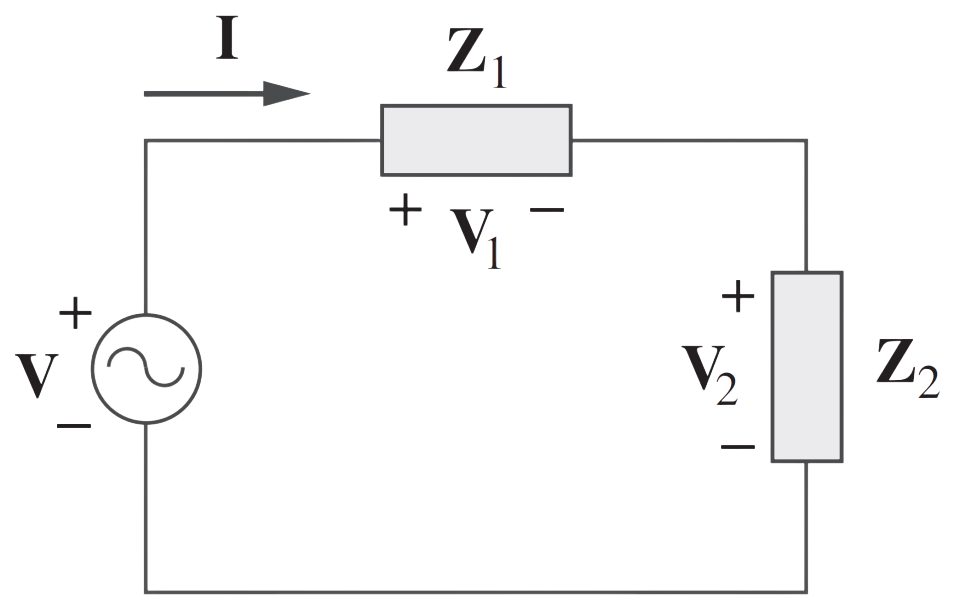
\includegraphics[width=0.5\linewidth]{zserie}\\
		$\textbf{\textit{V}}=\textbf{\textit{V}}_{1} +\textbf{\textit{V}}_{2}+....\textbf{\textit{V}}_{n} =\textbf{\textit{I}}.(\textbf{\textit{Z}}_{1} +\textbf{\textit{Z}}_{2}+....\textbf{\textit{Z}}_{n}) $\\
		\vspace{0.1cm}		
		$\textit{\textbf{Z}}_{eq}=\dfrac{\textbf{\textit{V}}}{\textbf{\textit{I}}}=\textbf{\textit{Z}}_{1} +\textbf{\textit{Z}}_{2} +\textbf{\textit{Z}}_{3} +....\textbf{\textit{Z}}_{n}$\\
		\vspace{0.1cm}	
		Divisor de tensión\\
		$\boxed{\textbf{\textit{V}}_{1}=\dfrac{\textbf{\textit{Z}}_{1}}{\textbf{\textit{Z}}_{1}+\textbf{\textit{Z}}_{2} } . \textbf{\textit{V}}}$		$\boxed{\textbf{\textit{V}}_{2}=\dfrac{\textbf{\textit{Z}}_{2}}{\textbf{\textit{Z}}_{1}+\textbf{\textit{Z}}_{2} } . \textbf{\textit{V}}}$
		$\boxed{\textbf{\textit{V}}_{n}=\textbf{\textit{Z}}_{n}.\textbf{\textit{I}}}$\\

		\vspace{0.6cm}
		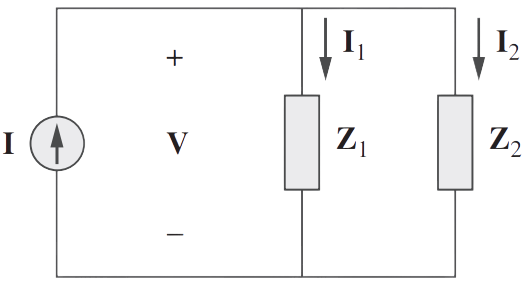
\includegraphics[width=0.5\linewidth]{zparalelo}\\	
		$\textbf{\textit{I}}=\textbf{\textit{I}}_{1} +\textbf{\textit{I}}_{2}+....\textbf{\textit{I}}_{n} =\textbf{\textit{V}}.(\dfrac{1}{\textbf{\textit{Z}}_{1}} +\dfrac{1}{\textbf{\textit{Z}}_{2}}+....+\dfrac{1}{\textbf{\textit{Z}}_{n}} ) $\\
		\vspace{0.1cm}
		$\textbf{\textit{Y}}_{eq}=\dfrac{1}{\textbf{\textit{Z}}_{eq}}=\dfrac{\textbf{\textit{I}}}{\textbf{\textit{V}}}=\dfrac{1}{\textbf{\textit{Z}}_{1}} +\dfrac{1}{\textbf{\textit{Z}}_{2}}+...+\dfrac{1}{\textbf{\textit{Z}}_{n}}$\\
				\vspace{0.1cm}	
		Divisor de corriente\\
		$\boxed{\textbf{\textit{I}}_{1}=\dfrac{\textbf{\textit{Z}}_{2}}{\textbf{\textit{Z}}_{1}+\textbf{\textit{Z}}_{2} } . \textbf{\textit{I}}}$		$\boxed{\textbf{\textit{I}}_{2}=\dfrac{\textbf{\textit{Z}}_{1}}{\textbf{\textit{Z}}_{1}+\textbf{\textit{Z}}_{2} } . \textbf{\textit{I}}}$
		$\boxed{\textbf{\textit{V}}=\textbf{\textit{Z}}_{n}.\textbf{\textit{I}}_{n}}$\\
	\end{center}

	\begin{tabular}{r | l} \vspace{.2cm}
		& \\ \vspace{.2cm}
		& \\ \vspace{.2cm}
		& \\ \vspace{.2cm}
		& \\ \vspace{.2cm}
		& \\ 
		
	\end{tabular}
	
	\unidad{4}{Respuesta Completa}
	
	
	\begin{tabular}{r | l} \vspace{.2cm}
		& \\ \vspace{.2cm}
		& \\ \vspace{.2cm}
		& \\ \vspace{.2cm}
		& \\ \vspace{.2cm}
		& \\ 
		
	\end{tabular}
	
	\unidad{5}{Potencia y Energía en Circuitos Monofásicos}
	
	
	\begin{tabular}{r | l} \vspace{.2cm}
		& \\ \vspace{.2cm}
		& \\ \vspace{.2cm}
		& \\ \vspace{.2cm}
		& \\ \vspace{.2cm}
		& \\ 
		
	\end{tabular}
	
	\unidad{6}{Redes Eléctricas}
	
	
	\begin{tabular}{r | l} \vspace{.2cm}
		& \\ \vspace{.2cm}
		& \\ \vspace{.2cm}
		& \\ \vspace{.2cm}
		& \\ \vspace{.2cm}
		& \\ 
		
	\end{tabular}
	
	\unidad{7}{Circuitos Polifásicos}
	
	
	\begin{tabular}{r | l} \vspace{.2cm}
		& \\ \vspace{.2cm}
		& \\ \vspace{.2cm}
		& \\ \vspace{.2cm}
		& \\ \vspace{.2cm}
		& \\ 
		
	\end{tabular}
	
	\unidad{8}{Circuitos Magnéticos y Acoplados}
	
	
	\begin{tabular}{r | l} \vspace{.2cm}
		& \\ \vspace{.2cm}
		& \\ \vspace{.2cm}
		& \\ \vspace{.2cm}
		& \\ \vspace{.2cm}
		& \\ 
		
	\end{tabular}
	
	\unidad{9}{Bloques y Funciones de Transferencia}
	
	
	\begin{tabular}{r | l} \vspace{.2cm}
		& \\ \vspace{.2cm}
		& \\ \vspace{.2cm}
		& \\ \vspace{.2cm}
		& \\ \vspace{.2cm}
		& \\ 
		
	\end{tabular}
	
	\unidad{10}{Circuitos No Lineales}
	
	
	\begin{tabular}{r | l} \vspace{.2cm}
		& \\ \vspace{.2cm}
		& \\ \vspace{.2cm}
		& \\ \vspace{.2cm}
		& \\ \vspace{.2cm}
		& \\ 
		
	\end{tabular}
	
	\unidad{11}{Componentes Simétricas}
	
	
	\begin{tabular}{r | l} \vspace{.2cm}
		& \\ \vspace{.2cm}
		& \\ \vspace{.2cm}
		& \\ \vspace{.2cm}
		& \\ \vspace{.2cm}
		& \\ 
		
	\end{tabular}
	
	
\end{document}